\documentclass[a4paper]{article}

\usepackage{listings}
\usepackage{graphicx}
\usepackage{tabularx}
\usepackage{tikzsymbols}
\usepackage{hyperref}
\usepackage{amsmath}
\usepackage{amssymb}

\usepackage[margin=2cm]{geometry}

\usepackage{titlesec}
\titleformat*{\section}{\large\bfseries}

\definecolor{kit-blue}{RGB}{70, 100, 170}
\input{../slides/l00-commands.tex}

\begin{document}
\exhead{3}{2024-06-03}{2024-06-17}

\newcommand{\statetilled}{T}
\newcommand{\statetobetilled}{$+$}
\newcommand{\statenottobetilled}{$-$}
\section{Competition: SDVSTP (8(+8) Points)}

Consider the well-known and industrially relevant \textit{Stardew Valley Soil Tilling Problem} (SDVSTP), which we also talked about (in a slightly simpler form) in the 0th exercise.
\\
We have a $w \times h$ 2D grid $G$ of ``soil'' cells. Each of the $w\cdot h$ cells is in exactly one of the following states: \emph{tilled} (\statetilled), \emph{should be tilled} (\statetobetilled), or \emph{must not be tilled} (\statenottobetilled).
We also define the following five \textit{patterns} (corresponding to five increasing \textit{charging levels} of a hoe):

\begin{figure}[h!]
	\centering
	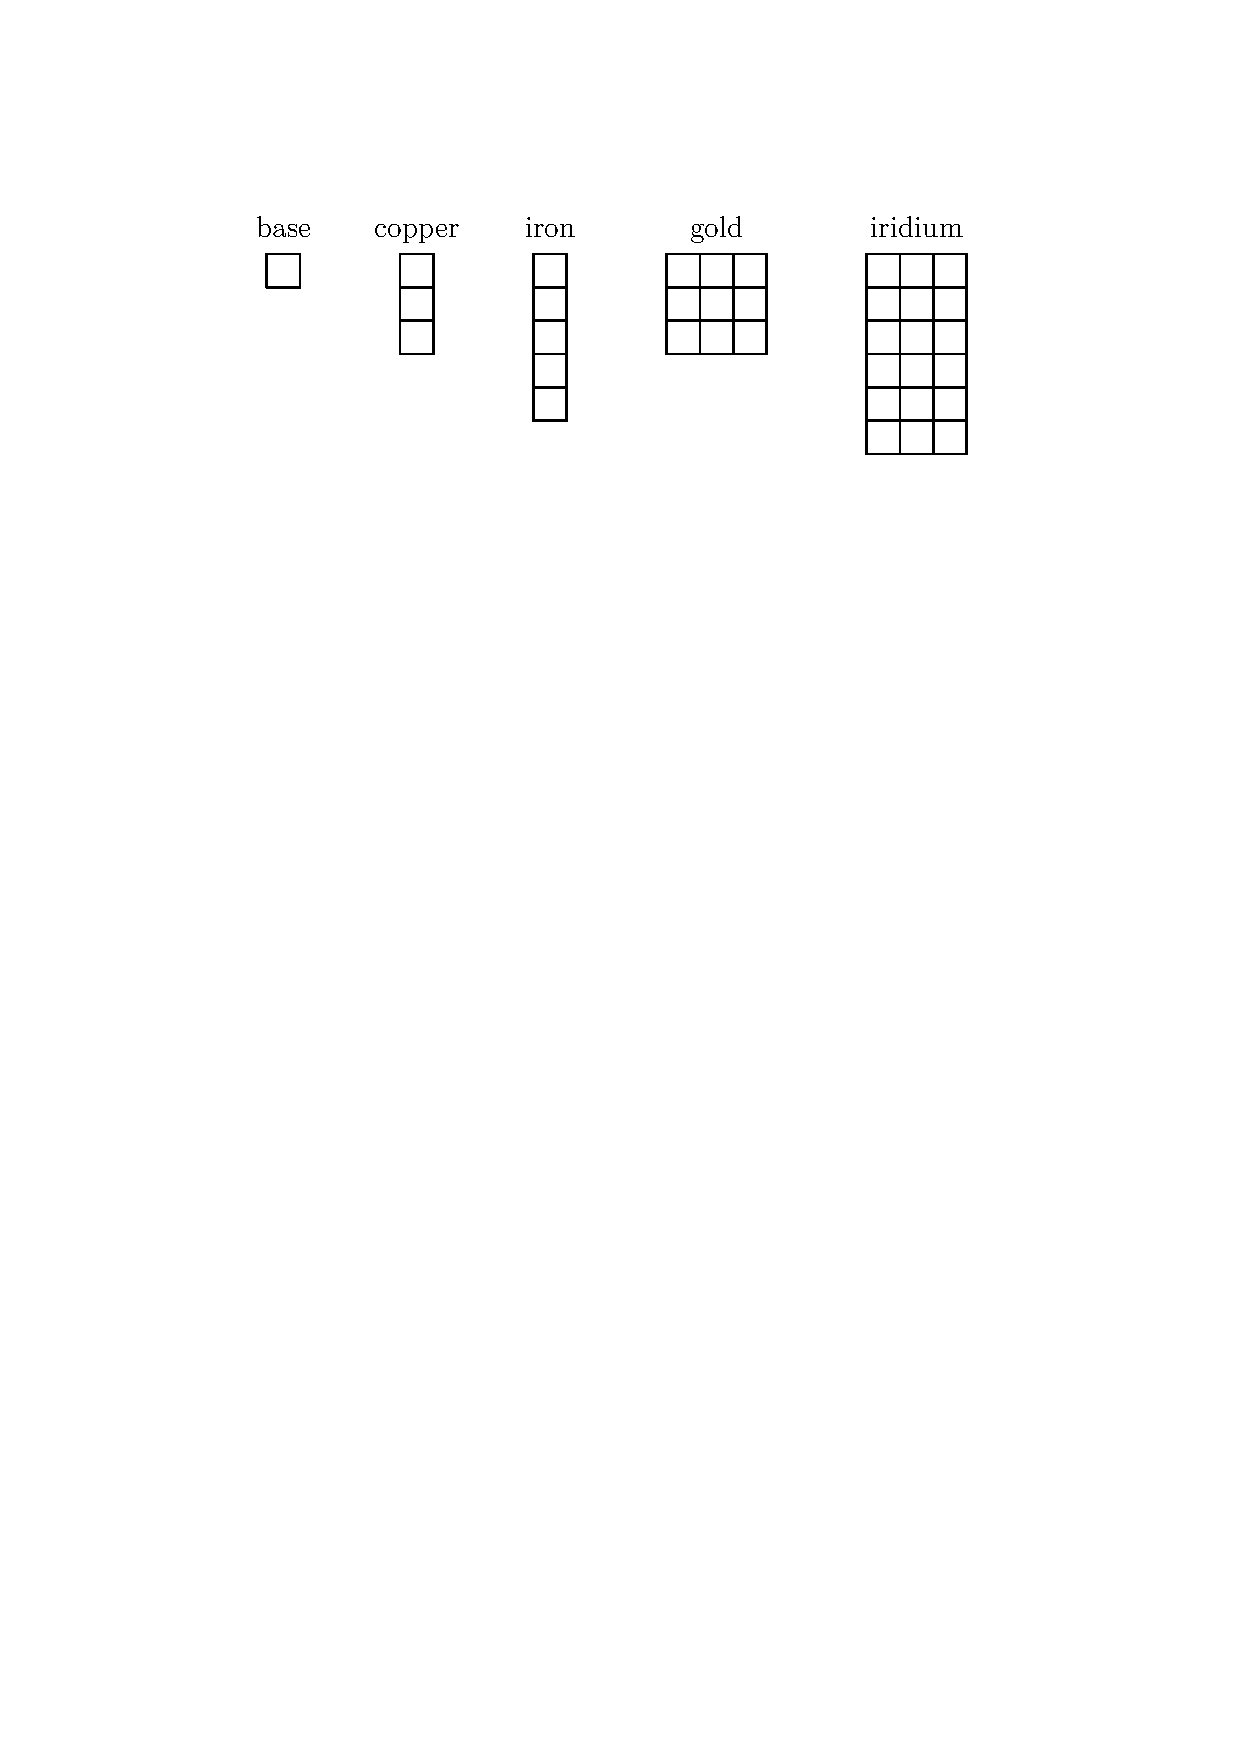
\includegraphics[width=0.475\textwidth]{figures/sdvstp-patterns.pdf}
\end{figure}
\noindent
We further define \emph{action} $a = (p,r,x,y)$ as follows: Rotate the pattern $p \in \{$base, copper, iron, gold, iridium$\}$ by $r \in \{0^\circ, 90^\circ\}$ and then align its \textit{upper left corner} with grid position $(x,y)$.
Then $a$ is \textit{applicable} if the pattern is fully contained within $G$.
Applying $a$ changes all cells in $G$ under the pattern to state \statetilled.

A \textit{solution} for $G$ is a set of applicable actions $A = \{ a_1, a_2, \ldots, a_k \}$ such that applying each action in $A$ transforms $G$ into the grid $G'$ where all cells that were initially in state \statetobetilled{} are in state \statetilled{} and all cells that were initially in state \statenottobetilled{} are still in state \statenottobetilled{}.
The objective is to find a solution that minimizes $k$.

Devise a SAT-based SDVSTP solver.
Your program should take a single argument, the path to an input file in the straight-forward \texttt{.sdvstp} format, structured as in the example in Fig.~\ref{fig:sdv-sol} (left).
The solver should output a line ``\texttt{s SOLUTION k}'', where $k$ is the minimum number of required actions, followed by $k$ lines describing each individual action $(p,r,x,y) \in A$, as in Fig.~\ref{fig:sdv-sol} (center).

\begin{figure}[h!]
	\begin{minipage}{0.33\textwidth}
		\begin{verbatim}
			p sdvstp 8 5
			++++++++
			++++++++
			++T--+++
			+TT--+++
			-------+
			
		\end{verbatim}
	\end{minipage}%
	\begin{minipage}{0.33\textwidth}
		\begin{verbatim}
			s SOLUTION 6
			v gold    0 0 0
			v gold    0 5 1
			v iron   90 3 0
			v copper 90 3 1
			v base    0 0 3
			v base    0 7 4
		\end{verbatim}
	\end{minipage}%
	\begin{minipage}{0.33\textwidth}
		\centering
		\vspace*{2mm}
		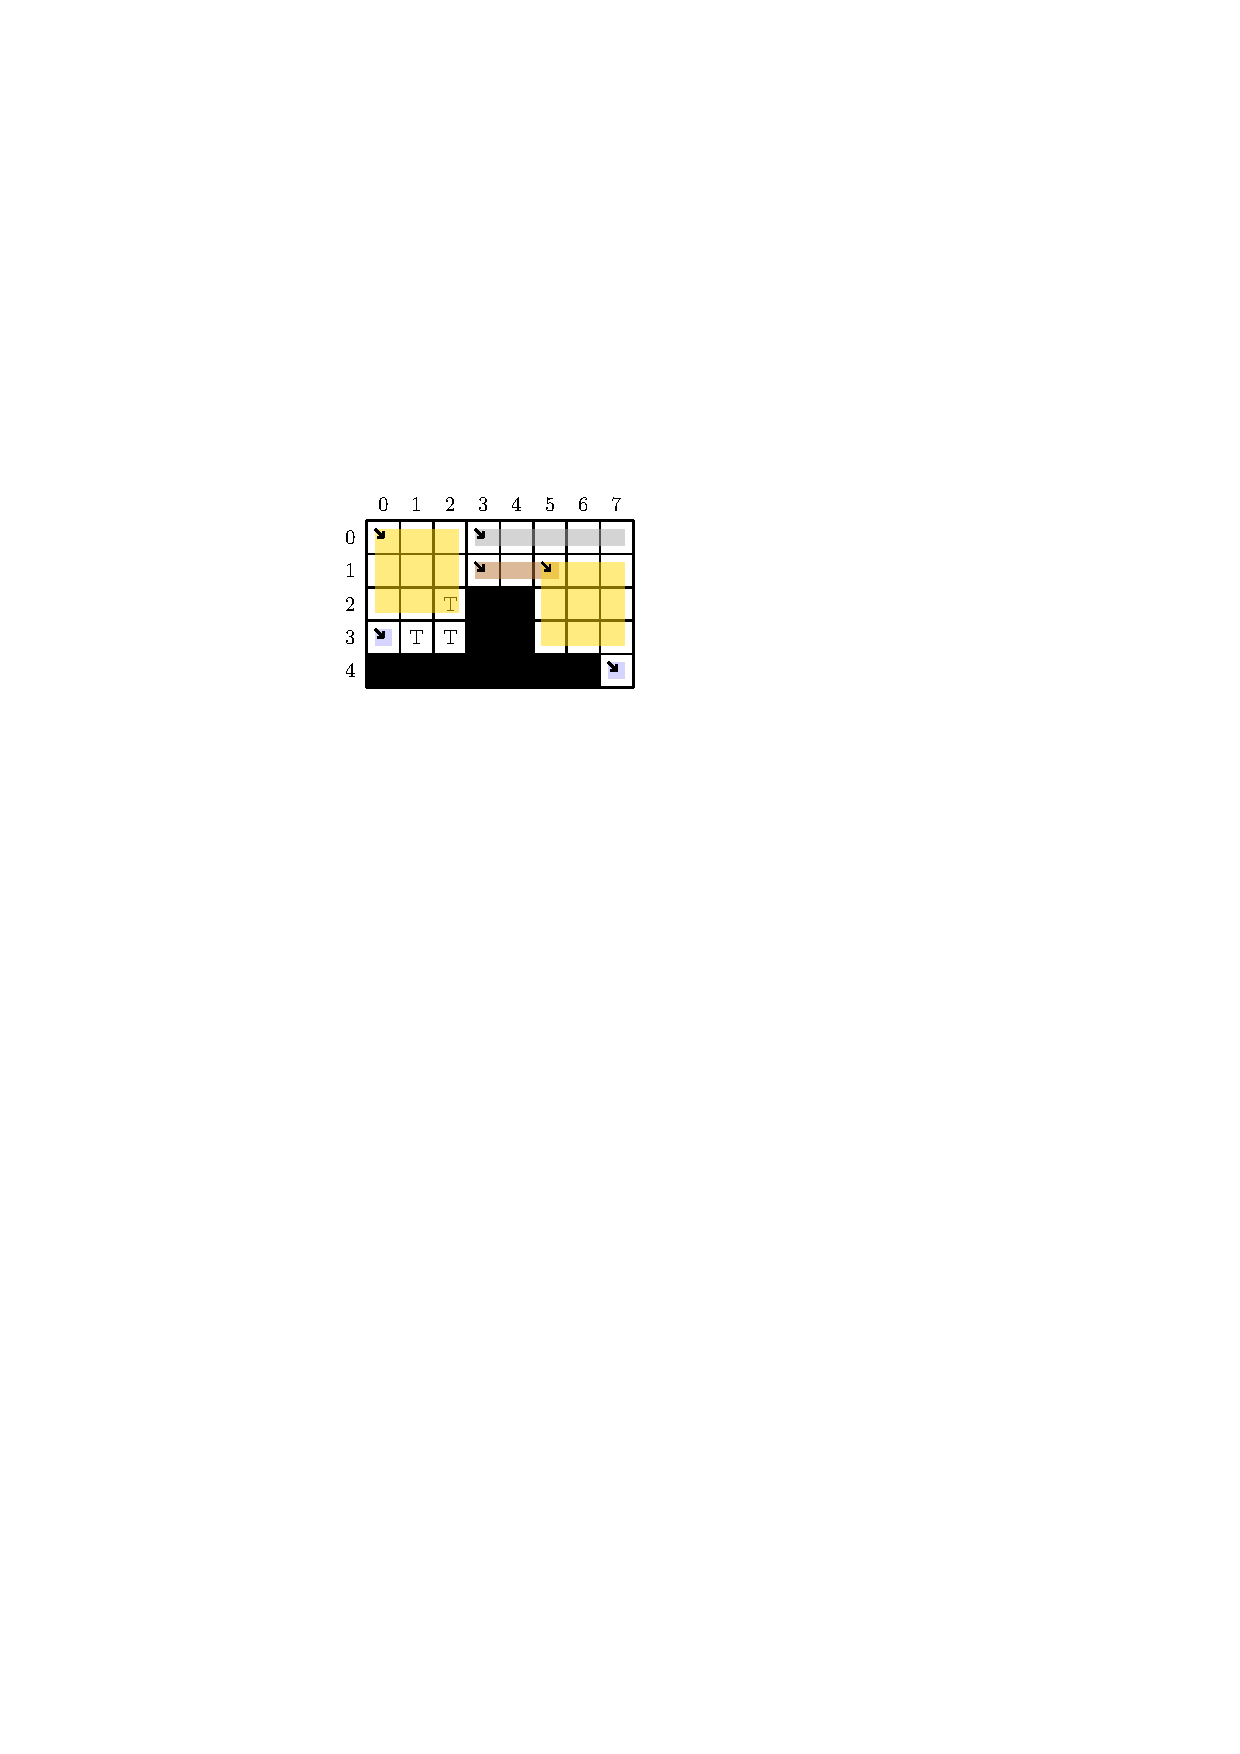
\includegraphics[width=0.8\textwidth]{figures/sdvstp-solution.pdf}\\[2mm]
		~
	\end{minipage}%
	\caption{Left: Example \texttt{.sdvstp} input file specifying an $8\times 5$ grid.
		Center: Possible corresponding output of the solver (columns aligned only for better readability).
		Right: illustration of the grid and the output solution, with the top-left ``anchor point'' of each pattern marked with an arrow.
	}
	\label{fig:sdv-sol}
\end{figure}

You get 8 points for a correct SDVSTP solver that is able to solve easy instances within a few minutes.
The best performing solution is awarded double the points.

\vspace*{3mm}
\noindent
\textbf{Code skeleton:} \url{https://github.com/satlecture/kit2025/blob/main/code/src/sdvstp/sdvstp.cc}~\\[1ex]
\noindent
\textbf{Some benchmark instances:} \url{https://github.com/satlecture/kit2025/tree/main/exercises/sdvstp}

\newpage

\section{CDCL (3+6 Points)}
\subsection{a)}
Simulate the CDCL algorithm by hand on the formula F. Select branching literals in the order $x_1,x_2,x_3, ...$. Draw the implication graph once a conflict occurs, learn the 1-UIP clause and continue CDCL search with the variable implied by the asserting learned clause. If everything goes right you should only encounter a single conflict before arriving a satisfying assignment. To emphasize the structure, each variable $x_i$ is just written as~$i$ and it's negation $\bar x_i$ as $-i$. So for example, $\bar x_4$ is written as $-4$ and $x_8$ as 8.
\begin{align}
	F = \{\{-1,-2,-4\}, \{-3, 6\}, \{-5,-6, 8\}, \{4,-8,10\}, \\ \{7,9\}, \{-2, -8, 9\}, \{-1,-9-10\},  \{-5,8,9\}\}
\end{align}

\subsection{b)}
Repeat the CDCL algorithm, now for the larger formula $F'$. Again, select branching literals again in the order $x_1,x_2,x_3, ...$. Draw the implication graph at every conflict and give the learned 1-UIP clause. Provide the final assignment.
\begin{align}
	\centering
	F' = &\{\{1, 13\}, \{-1, -2, 14\}, \{3, 15\}, \{4, 16\},\{-5, -3, 6\},  \notag \\
	\quad & \{-5, -7\}, \{-6, 7, 8\}, \{-4, -8, -9\}, \{-1, 9, -10\},\notag \\
	\quad & \{9, 11, -14\}, \{10, -11, 12\}, \{-2, -11, -12\}\}
\end{align}






\section{Competition: Autarkies ($7 (+7)$ Points)}
Write an anytime algorithm that computes a maximal autarky for a given formula, i.e., an autarky that satisfies as many clauses as possible.
The tool should accept a DIMACS file path as input and, as soon as possible, output a set of literals representing an autarky. 
Then, it should output improved sets iteratively.
For each autarky, use a single line that begins with "v~" and ends with a zero, with space-separated literals of the autarky in between. This format is similar to the SAT Competition Solution Output Format [1].\\

\noindent
We will run your submission on DIMACS files and evaluate the quality of the solutions found within a set time limit.
We will stop each run after $k$ minutes.
Then, we will check the last output line to see if it contains a valid autarky and compute the number of clauses satisfied by the autarky.
The solution that finds the best autarkies on average will win the competition.\\

\noindent
[1] \textbf{Output Format:} \url{https://satcompetition.github.io/2025/output.html}


\section{Variable Elimination ($3$ Points)}
For a gate encoding $E$ with output $x$ in a formula $F = E \cup R$,
we simplified the resolvents $(E_x \cup R_x) \otimes (E_{\overline x} \cup R_{\overline x})$ by
$S := (E_x \otimes R_{\overline x}) \cup (R_x \otimes E_{\overline x})$, dropping both
$R_x \otimes R_{\overline x}$ and $E_x \otimes E_{\overline x}$.
Show that the clauses in $R_x \otimes R_{\overline x}$ can be derived from $S$ by resolution.
You can assume that $E$ encodes a binary AND gate.


\section{Variable Elimination ($2 \times 2$ Points)}
Let the formula $S$ with gate encodings $E_1$ and $E_2$ be given.
Apply variable elimination for gates for variables $a$ and $r$.
Give the clause sets after each elimination step.
Try the following two strategies.

\begin{enumerate}\setlength{\itemsep}{0pt}
\item Eliminate variable $a$ first, and then $r$ if possible.
\item Eliminate variable $r$ first, and then $a$ if possible.
\end{enumerate}
\vspace*{-1ex}
\begin{align*}
S = \bigl\{ \underbrace{\{ \lnot x, \lnot y, a \}, \{ x, \lnot a \}, \{ y, \lnot a \}}_{E_1},
\underbrace{\{ \lnot a, r \}, \{ \lnot z, r \}, \{ a, z, \lnot r \}}_{E_2}, \{ a, z, r \},
\{ \lnot a, \lnot r \} \bigr\}
\end{align*}


\section{Blocked Clauses ($3\times 3$ Points)}
If Blocked Clause Elimination (BCE) reduces a formula $F$ to the empty formula then $F$ is called a blocked set.
Prove the following statements.

\begin{enumerate}\setlength{\itemsep}{0pt}
	\item Any formula $F$ can be partitioned into two blocked sets $S$ and $L$ such that $F = S\cup L$.
    Design a linear algorithm that produces $L$ and $S$ from $F$.
	\item Blocked sets are not closed unter resolution. 
    If $F$ is a blocked set then $F \cup C_1 \otimes C_2$, where $C_1,C_2 \in F$ may not be a blocked set anymore.
	\item Blocked sets are not closed unter partially assigning variables.
    If $F$ is a blocked set then $F_{x=v}$ (the result of assigning $v$ to $x$ and subsequent simplification) may not be a blocked set anymore.
\end{enumerate}

\end{document}